\documentclass{article}

% --- Codificación / idioma ---
\usepackage[T1]{fontenc}
\usepackage[utf8]{inputenc} % (pdfLaTeX)
\usepackage[spanish,es-tabla]{babel}
%\usepackage{microtype}

% --- Matemática / tablas / figuras ---
\usepackage{amsmath,amssymb,amsfonts,amsthm}
\usepackage{graphicx}
\usepackage{booktabs}
\usepackage{siunitx}
\sisetup{output-decimal-marker=.,detect-all}
\usepackage{enumitem}
\usepackage{multicol}
\setlength{\columnsep}{0.5cm}
\usepackage[margin=2cm]{geometry}

% --- Bibliografía ---
\usepackage{csquotes} % Cargar ANTES de biblatex
\usepackage[
  backend=biber,
  style=numeric,
  sorting=none,
  giveninits=true,
  maxnames=6,
  doi=false,
  isbn=false,
  url=false
]{biblatex}
\addbibresource{bibliografia.bib}

% --- Enlaces y referencias cruzadas ---
\usepackage[hidelinks]{hyperref}
\usepackage[capitalize,nameinlink]{cleveref}

% (Opcional) Traducciones de biblatex al español
\DefineBibliographyStrings{spanish}{andothers={et al.}}

\newcommand{\capconst}[1]{\par\smallskip\textit{Constantes: }#1}
% Teoremas
\newtheorem{theorem}{Teorema}[section]
\theoremstyle{definition}
\newtheorem{definition}{Definición}[section]
\newtheorem{proposition}{Proposición}[section]
\newtheorem{exercise}{Ejercicio}[section]
\theoremstyle{remark}
\newtheorem*{example}{\textbf{Ejemplos}}


\title{Informe 1, Laboratorio II - Ondas estacionarias.}
\author{%
\begin{tabular}{cc}
\multicolumn{2}{c}{\textbf{Profesor: Paulraj Manidurai}} \\
Fabián Contreras Muñoz & José Rosas Sepúlveda \\
Javier Chandia Valdés & Mario Díaz San Martín \\
\multicolumn{2}{c}{Martin Fierro Sagredo.}
\end{tabular}
}
\date{08/09/2025}
\begin{document}
\maketitle
% La regla va fuera de \author:
\noindent\makebox[\linewidth]{\rule{1\linewidth}{0.4pt}}\par\vspace{0.3cm}


\begin{abstract}
Se determinó la \textbf{densidad lineal} de cuerdas de \textbf{algodón}, \textbf{goma delgada} y \textbf{goma gruesa} mediante \textbf{ondas estacionarias} en un montaje con \textbf{parlante, polea y masas}. Se aplicaron dos protocolos: \textbf{tensión variable} (frecuencia fija) y \textbf{frecuencia variable} (tensión fija). Se utilizaron \textbf{seis cuerdas} en total (dos por material, una por protocolo), por lo que los resultados se interpretaron \textbf{por material/protocolo} y no como \textbf{comparación directa entre métodos}. A partir de \textbf{ajustes lineales} se estimó la densidad y se contrastó con la \textbf{estimación geométrica} (masa/longitud): en general hubo \textbf{concordancia de orden de magnitud}, con mayores \textbf{discrepancias en cuerdas de goma} atribuibles a \textbf{extensibilidad} y \textbf{fricción} del montaje.
\end{abstract}

\begin{multicols}{2}[\section*{Objetivos}]
\subsubsection*{Objetivo general}
\begin{itemize}[leftmargin=*, itemsep=2pt]
  \item Estimar la densidad lineal $\mu$ de cuerdas de algodón, goma delgada y goma gruesa usando ondas estacionarias.
\end{itemize}

\subsubsection*{Objetivos específicos}
\begin{enumerate}[leftmargin=*, itemsep=2pt, label=\textbf{\arabic*.}]
  \item Aplicar dos protocolos: \textbf{tensión variable} (con $\nu$ fija) y \textbf{frecuencia variable} (con $T$ fija), asignando \emph{una muestra distinta por protocolo} para cada material (total: seis cuerdas).
  \item Para cada muestra, extraer $\mu$ a partir de la pendiente del ajuste lineal correspondiente y contrastarla con la estimación geométrica $\mu_{0}=m/L$ de esa misma muestra.
  \item Discutir limitaciones del modelo ideal (fricción en polea, extensibilidad, definición de $L$ efectivo) y su impacto en las estimaciones.
\end{enumerate}
\end{multicols}



\begin{multicols}{2}
[\section*{Introducción}]

\paragraph{Contexto histórico.}
El estudio de las ondas en cuerdas tensas se consolidó a mediados del siglo XVIII con los trabajos de d’Alembert, Euler y Bernoulli sobre la ecuación de ondas y los modos normales; más tarde, experimentos como el de Melde (siglo XIX) ilustraron la formación de \emph{ondas estacionarias} por superposición de ondas viajeras con igual amplitud y frecuencia en sentidos opuestos \parencite{FeynmanI49,BritannicaStandingWaves,MeldeWiki}.

\paragraph{Marco teórico mínimo.}
Para una cuerda fija en $x=0$ y $x=L$ (condiciones de borde $y(0,t)=y(L,t)=0$), la superposición de dos ondas viajeras
\begin{equation*}
y(x,t)=A\sin(kx-\omega t)+A\sin(kx+\omega t)
\end{equation*}
genera el patrón estacionario
\begin{equation}
y(x,t)=2A\cos(\omega t)\sin(kx)\,, \label{eqcuerda}
\end{equation}
en el que los nodos satisfacen $y(x_n,t)=0$ para todo $t$ \parencite{OpenStax16-2,MIT8.03Lec9}.

\paragraph{Nodos, antinodos y cuantización.}
De $y(x_n,t)=0$ se sigue
\begin{equation*}
\sin(kx_n)=0 \;\Longrightarrow\; kx_n=n\pi \quad (n\in\mathbb{N})\,,
\end{equation*}
de modo que
\begin{equation*}
k_n=\frac{n\pi}{L}\,, \qquad \lambda_n=\frac{2\pi}{k_n}=\frac{2L}{n}\,.
\end{equation*}
En este contexto $n$ coincide con el número de \emph{antinodos} del modo $n$ \parencite{OpenStax16-6,FeynmanI49}.

\paragraph{Frecuencias permitidas.}
Si la velocidad de fase de las ondas en la cuerda es $v$ y $\nu$ denota la frecuencia, se cumple $v=\lambda \nu$. Por tanto, las frecuencias de los modos estacionarios son
\begin{equation}
\nu_n=\frac{v}{\lambda_n}=\frac{n}{2L}\,v
=\frac{n}{2L}\sqrt{\frac{T}{\mu}}\,, \label{eqnun}
\end{equation}
donde $T$ es la tensión y $\mu$ la densidad lineal de masa \parencite{OpenStax16-6,HyperPhysicsString,MIT8.03Lec9}. La relación \eqref{eqnun} es la base de los dos protocolos experimentales que usaremos más adelante: uno con $T$ fija (variando $\nu$) y otro con $\nu$ fija (variando $T$).
\end{multicols}
newpage
\begin{multicols}{2}
[\subsection*{Relaciones operativas para extraer \texorpdfstring{$\mu$}{mu}}]

En una cuerda tensa la velocidad de fase cumple
\begin{align}
    v^{2}=\frac{T}{\mu}\,, \label{eqv2}
\end{align}
donde \(T\) es la \textbf{tensión} y \(\mu\) la \textbf{densidad lineal de masa} \parencite{OpenStax16-6,MIT8.03Lec9}. Combinando \eqref{eqv2} con \eqref{eqnun}, se obtienen las relaciones de trabajo:
\begin{align*}
    \nu_{n}^{2}&=\frac{n^{2}\,T}{4L^{2}\mu}\,,\\
    T_{n}&=\frac{4L^{2}\,\nu^{2}}{n^{2}}\,\mu\,,
\end{align*}
que vinculan las magnitudes medibles con \(\mu\). Aquí \(\nu_{n}\) y \(T_{n}\) son los valores \emph{por modo} (variables entre puntos), mientras que \(\nu\) o \(T\) se mantienen \textbf{fijos} según el protocolo aplicado.

Estas expresiones sustentan los dos procedimientos experimentales: con \textbf{\(T\) fija} se grafica \(\nu\) vs.\ \(n\) (pendiente \(\propto \sqrt{T/\mu}\)); con \textbf{\(\nu\) fija} se grafica \(T\) vs.\ \(1/n^{2}\) (pendiente \(\propto L^{2}\nu^{2}\mu\)). El \textbf{largo efectivo} \(L\), la \textbf{frecuencia} \(\nu\), la \textbf{tensión} \(T\) y el \textbf{número de antinodos} \(n\) son accesibles experimentalmente.
\end{multicols}

\begin{multicols}{2}[\section*{Experimento}]

\subsection*{Materiales}
\begin{itemize}
\item Generador de frecuencias.
\item Parlante vibrador (forzador).
\item Cables tipo banana.
\item Conjunto de masas y gancho metálico (colgante).
\item Regla de 1.50 metros.
\item Barra y soporte vertical.
\item Polea con soporte y prensa.
\item Carrete con hilo de algodón.
\item Balanza.
\item Cuerdas de goma (Poliuretano PASCO).
\end{itemize}

\subsection*{Procedimiento general}
Se comienza con el sistema armado como en el esquema de la \cref{fig:montaje1}. Todas las magnitudes se reportan en el \textbf{Sistema Internacional (SI)}.
\begin{enumerate}[label=\textbf{\arabic*.}, leftmargin=*]
\item Medir la \textbf{longitud total} y la \textbf{masa} de cada cuerda para obtener una estimación geométrica de la densidad lineal, $\mu_0=m/L$.
\item Fijar la \textbf{longitud efectiva} del tramo vibrante en $L\approx\SI{1.00}{m}$ (entre el punto de sujeción en el parlante y el punto de contacto en la polea). La porción sobrante (10–50 cm) queda fuera del tramo vibrante.
\item Medir por separado la \textbf{masa del gancho} ($m_{\text{gancho}}$); al calcular la tensión usar $T=(M+m_{\text{gancho}})g$, donde $M$ es la masa colgante.
\item \textbf{Montaje mecánico.} Fijar un extremo de la cuerda al ojal/perno del \textbf{parlante vibrador}. Conducir el otro extremo \textbf{sobre la polea} y amarrarlo firmemente al \textbf{gancho portamasa}.\\
\emph{Protocolos:} en \textbf{tensión variable} mantener $\nu$ fija y \textbf{variar $M$} para alcanzar diferentes modos; en \textbf{frecuencia variable} mantener $M$ (y por tanto $T$) \textbf{constante} y barrer $\nu$. Verificar que el tramo vibrante quede recto y a nivel, con el menor rozamiento posible en la polea.
\item Ajustar en el generador la \textbf{amplitud mínima} necesaria para visualizar claramente los antinodos, evitando no linealidades.
\end{enumerate}

\end{multicols}

\begin{figure}
    \centering
    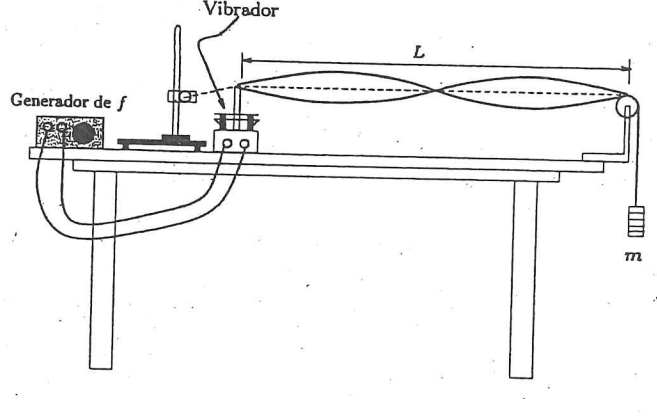
\includegraphics[width=0.5\linewidth]{imagenes/setup.png}
    \caption{Montaje del experimento.\capconst{$g=\SI{9.81}{m/s^2}$, $m_{\text{gancho}}=\ldots$, $L=\ldots$}}%
    \label{fig:montaje1}
\end{figure}

\begin{multicols}{2}
\subsection*{Procedimiento: Tensión variable (\(\nu\) fija)}
\begin{enumerate}[label=\textbf{\arabic*.}, leftmargin=*]
\item Seleccionar una masa inicial relativamente grande (p.\,ej., \(m\approx\SI{0.25}{kg}\)) para garantizar tensión suficiente.
\item Con \(\nu\) fija, ajustar la frecuencia hasta identificar claramente un modo con \(n\) antinodos (idealmente, desde el fundamental \(n=1\) y hasta \(n\approx 8\); o, en casos particulares, como se verá más adelante, comenzando en un modo alto y descendiendo al fundamental).
\item Manteniendo \(\nu\) fija, \textbf{variar la masa} (quitando o añadiendo) y registrar \((n, m)\) cada vez que se estabilice un modo estacionario. Usar \(T=(m+m_{\text{gancho}})g\).
\end{enumerate}

\subsection*{Procedimiento: Frecuencia variable (\(T\) fija)}
\begin{enumerate}[label=\textbf{\arabic*.}, leftmargin=*]
\item Elegir una masa fija (p.\,ej., \(m\leq\SI{0.35}{kg}\)) y, por tanto, una tensión fija \(T=(m+m_{\text{gancho}})g\).
\item Barrer la frecuencia \(\nu\) para localizar el primer modo (fundamental) y anotar \((n=1,\nu_1)\).
\item Continuar variando \(\nu\) y registrar \((n,\nu_n)\) cada vez que aparezca un nuevo antinodo (modos \(n=2,3,\dots\)).
\end{enumerate}
\end{multicols}


\section*{Resultados y Cálculos}
\begin{multicols}{2}

\noindent\textbf{Advertencia metodológica.} Los dos protocolos (tensión variable a $\nu$ fija y frecuencia variable a $T$ fija) no se aplicaron sobre la misma cuerda. Por ello, \emph{no} se comparan métodos en una misma muestra; para cada cuerda se reporta únicamente el protocolo efectivamente realizado y su contraste con $\mu_{0}=m/L$.

\subsection*{Cuerda de algodón}
Se presentan los resultados para la cuerda de algodón. Para \textbf{tensión variable}, se presentan la Tabla \ref{tab:tension1} y la Figura \ref{fig:tension1}; para \textbf{frecuencia variable}, la Tabla \ref{tab:frecuencia1} y la Figura \ref{fig:frecuencia1}. Los valores estimados de densidad lineal fueron:
\begin{align*}
\mu_{0} &\approx 3.0\cdot10^{-4} \\
\mu(\nu) &\approx 2.5\cdot10^{-4} \\
\mu(T) &\approx 2.0\cdot10^{-4}
\end{align*}
donde $\mu_{0}$ es la estimación geométrica (masa/longitud), $\mu(T)$ proviene de la pendiente del ajuste en el gráfico de tensión variable, y $\mu(\nu)$ del ajuste en el gráfico de frecuencia variable.

\subsection*{Cuerda de goma delgada}
En este caso, para \textbf{tensión variable}, se presentan la Tabla \ref{tab:tension2} y la Figura \ref{fig:tension2}; para \textbf{frecuencia variable}, la Tabla \ref{tab:frecuencia2} y la Figura \ref{fig:frecuencia2}. Se obtuvieron:
\begin{align*}
\mu_{0} &\approx 5.1\cdot10^{-3} \\
\mu(T) &\approx 3.1\cdot10^{-3} \\
\mu(\nu) &\approx 5.1\cdot10^{-3}
\end{align*}

\subsection*{Cuerda de goma gruesa}
Para \textbf{tensión variable}, se presentan la Tabla \ref{tab:tension3} y la Figura \ref{fig:tension3}; para \textbf{frecuencia variable}, la Tabla \ref{tab:frecuencia3} y la Figura \ref{fig:frecuencia3}. Los resultados fueron:
\begin{align*}
\mu_{0} &\approx 1.23\cdot10^{-2} \\
\mu(T) &\approx 7.5\cdot10^{-3} \\
\mu(\nu) &\approx 7.2\cdot10^{-3}
\end{align*}

\end{multicols}

\begin{figure}[htbp]
  \centering
  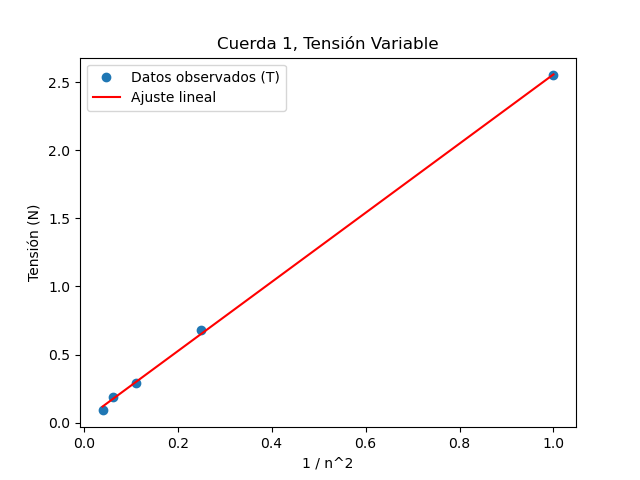
\includegraphics[width=0.55\linewidth]{imagenes/tension_variable_1.png}
  \caption{Tensión variable — Cuerda de algodón. Se grafica $T$ [N] en función de $1/n^{2}$ con $\nu$ fija; el ajuste lineal $T=a\,(1/n^{2})$ permite estimar $\mu$ vía $a=4L^{2}\nu^{2}\mu$.%
  \capconst{$L=\SI{9e-1}{m}$, $\nu=\SI{62}{Hz}$, $m_{\text{gancho}}=\SI{10e-3}{kg}$, $a=\SI{4.19}{N}$, $\mu=\SI{3.03e-3}{kg/m}$}}
  \label{fig:tension1}
\end{figure}

\begin{figure}
  \centering
  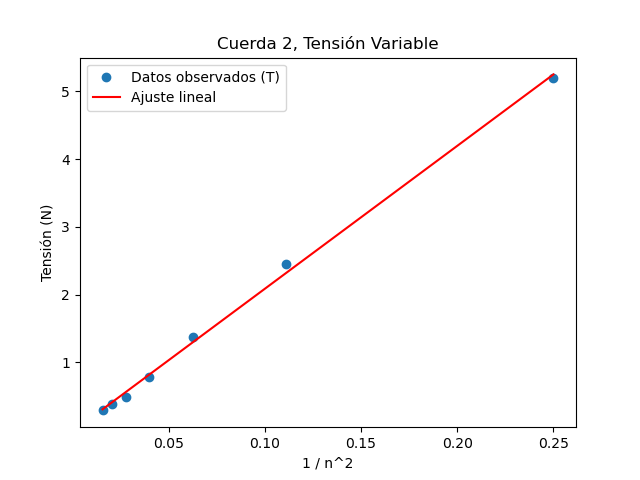
\includegraphics[width=0.55\linewidth]{imagenes/tension_variable_2.png}
  \caption{Tensión variable — Cuerda de goma delgada. $T$ [N] vs.\ $1/n^{2}$ a $\nu$ fija; pendiente $a$ tal que $a=4L^{2}\nu^{2}\mu$.%
  \capconst{$L=\SI{1.00}{m}$, $\nu=\SI{41.1}{Hz}$, $m_{\text{gancho}}=\SI{1.114e-3}{kg}$, $a=\SI{20.94}{N}$, $\mu=\SI{3.1e-3}{kg/m}$}}
  \label{fig:tension2}
\end{figure}

\begin{figure}
  \centering
  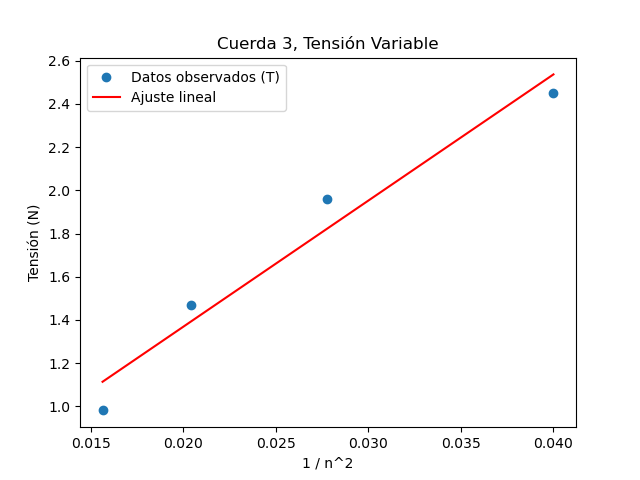
\includegraphics[width=0.55\linewidth]{imagenes/tension_variable_3.png}
  \caption{Tensión variable — Cuerda de goma gruesa. $T$ [N] vs.\ $1/n^{2}$ a $\nu$ fija; la pendiente $a$ determina $\mu$ mediante $a=4L^{2}\nu^{2}\mu$.%
  \capconst{$L=\SI{1.00}{m}$, $\nu=\SI{46.6}{Hz}$, $m_{\text{gancho}}=\SI{1.114e-3}{kg}$, $a=\SI{65.22}{N}$, $\mu=\SI{7.5e-3}{kg/m}$}}
  \label{fig:tension3}
\end{figure}


%%%%%%%%%%%%%%%%%%%5
%FRECUENCIAS
%%%%%%%%%%%%%%%%%%%%
\begin{figure}
  \centering
  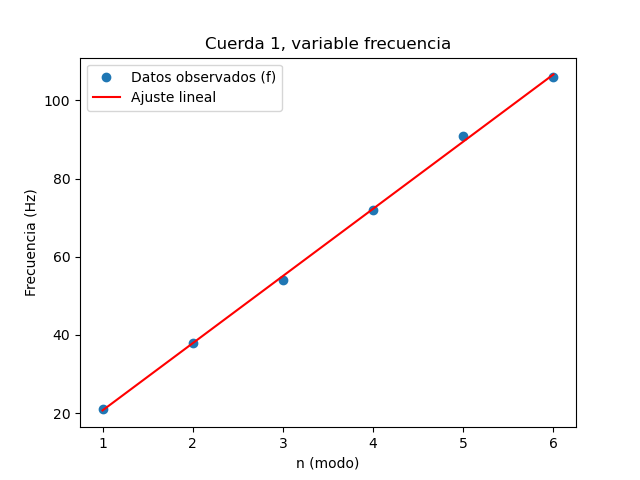
\includegraphics[width=0.55\linewidth]{imagenes/frecuencia_variable_1.png}
  \caption{Frecuencia variable — Cuerda de algodón. Se grafica $\nu$ [Hz] en función de $n$ con $T$ fija; el ajuste lineal $\nu=m\,n$ permite estimar $\mu$ con $m=\tfrac{1}{2L}\sqrt{T/\mu}$.%
  \capconst{$L=\SI{1.00}{m}$, $T=\SI{2.97e-2}{N}$, $m_{\text{gancho}}=\SI{10.3e-4}{kg}$, $M=\SI{2.0e-2}{kg}$, $\mu=\SI{2.7e-4}{kg/m}$}}
  \label{fig:frecuencia1}
\end{figure}

\begin{figure}
  \centering
  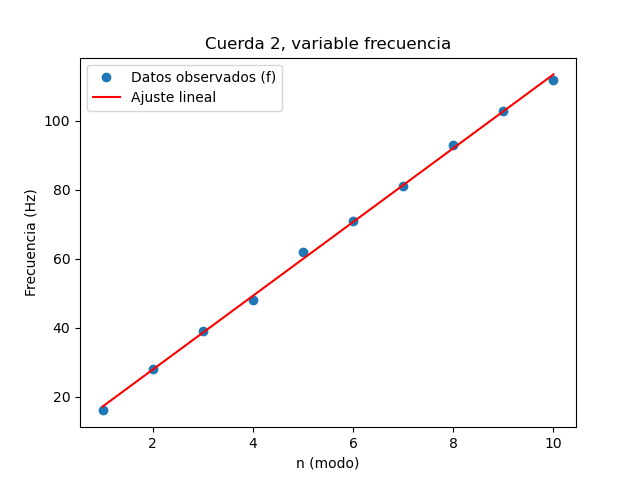
\includegraphics[width=0.55\linewidth]{imagenes/frecuencia_variable_2.png}
  \caption{Frecuencia variable — Cuerda de goma delgada. $\nu$ [Hz] vs.\ $n$ a $T$ fija; pendiente $m$ tal que $m=\tfrac{1}{2L}\sqrt{T/\mu}$.%
  \capconst{$L=\SI{1.00}{m}$, $T=\SI{23.52}{N}$, $m_{\text{gancho}}=\SI{10e-4}{kg}$, $M=\SI{230e-2}{kg}$, $\mu=\SI{5.24e-3}{kg/m}$}}
  \label{fig:frecuencia2}
\end{figure}

\begin{figure}[htbp]
  \centering
  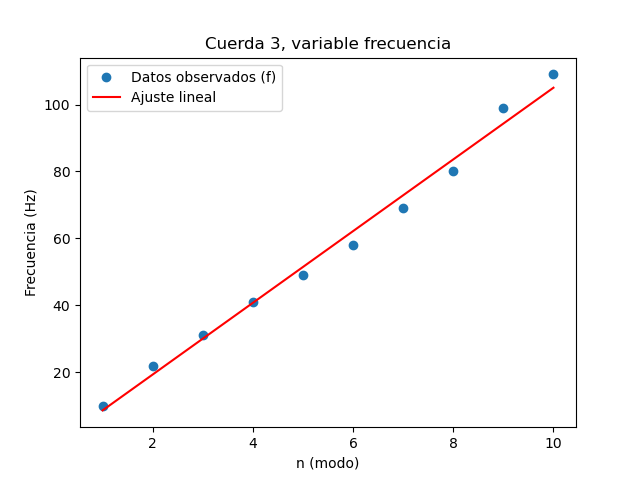
\includegraphics[width=0.55\linewidth]{imagenes/frecuencia_variable_3.png}
  \caption{Frecuencia variable — Cuerda de goma gruesa. $\nu$ [Hz] vs.\ $n$ a $T$ fija; la pendiente $m$ determina $\mu$ mediante $m=\tfrac{1}{2L}\sqrt{T/\mu}$.%
  \capconst{$L=\SI{1.00}{m}$, $T=\SI{33.32}{N}$, $m_{\text{gancho}}=\SI{10e-4}{kg}$, $M=\SI{330e-2}{kg}$, $\mu=\SI{1.35e-2}{kg/m}$}}
  \label{fig:frecuencia3}
\end{figure}



\begin{table}[htbp]
    \centering
    \begin{tabular}{c|c|c|c|c}
        Modo $n$ & $1/n^2$ & Tensión & Tensión esperada & Error porcentual (\%)\\
        \hline
        1 & 1 & 2.55 & 3.77 & 32.5 \\
        2 & 1/4 & 0.68 & 0.94 & 28 \\
        3 & 1/9 & 0.29 & 0.41 & 30 \\
        4 & 1/16 & 0.19 & 0.23 & 19 \\
        5 & 1/25 & 0.09 & 0.15 & 40  
    \end{tabular}
    \caption{Tensión Variable, Cuerda de Algodón (eliminando)}
    \label{tab:tension1}
\end{table}
\begin{table}[htbp]
    \centering
    \begin{tabular}{c|c|c|c|c}
        Modo $n$ & $1/n^2$ & Tensión & Tensión esperada & Error porcentual (\%)\\
        \hline
        2 & 1/4 & 5.19 & 8.73 & 40\\
        3 & 1/9 & 2.45 & 3.88 & 36\\
        4 & 1/16 & 1.37 & 2.18 & 37\\
        5 & 1/25& 0.78 & 1.39 & 44\\
        6 & 1/36 & 0.49 & 0.97 & 49\\
        7 & 1/49& 0.39 & 0.71 & 45\\
        8 & 1/64 & 0.29 & 0.54 & 46    
    \end{tabular}
    \caption{Cuerda de goma delgada (sumando)}
    \label{tab:tension2}
\end{table}
\begin{table}[htbp]
    \centering
    \begin{tabular}{c|c|c|c|c}
        Modo $n$ & $1/n^2$ & Tensión & Tensión esperada & Error porcentual (\%)\\
        \hline
        5 & 1/25 & 2.45 & 3.82 & 35\\ 
        6 & 1/36 & 1.96 & 2.65 & 26\\
        7 & 1/49 & 1.47 & 1.95 & 24\\
        8 & 1/64 & 0.98 & 1.49 & 34
    \end{tabular}
    \caption{Tensión Variable, Cuerda de goma Gruesa (sumando)}
    \label{tab:tension3}
\end{table}
%Ahora vienen las tablas para las frecuencias variables
\begin{table}[htbp]
    \centering
    \begin{tabular}{c|c|c|c}
        Modo $n$ & Frecuencia $\nu$ $[Hz]$ observada & Frecuencia $\nu$ $[Hz]$ esperada & Diferencia porcentual ($\%$) \\
        \hline
        1 & 21 & 15   & 34.1\\
        2 & 38 & 31 & 21.4\\
        3 & 55 & 46 & 15.0\\
        4 & 72 & 62 & 15.0\\
        5 & 91 & 78 & 16.3\\
        6 & 106 & 93 & 12.8
    \end{tabular}
    \caption{Cuerda de algodón, frecuencia variable.}
    \label{tab:frecuencia1}
\end{table}

\begin{table}[htbp]
    \centering
    \begin{tabular}{c|c|c|c}
        Modo $n$ & Frecuencia $\nu$ $[Hz]$ observada & Frecuencia $\nu$ $[Hz]$ esperada & Diferencia porcentual ($\%$) \\
        \hline
        1 & 16 & 10 & 50.3\\
        2 & 28 & 21 & 31.5\\
        3 & 39 & 31 & 22.1\\
        4 & 51 & 42 & 12.7\\
        5 & 62 & 53 & 16.4\\
        6 & 71 & 63 & 11.1\\
        7 & 81 & 74 & 8.7\\
        8 & 93 & 85 & 9.2\\
        9 & 103 & 95 & 7.5\\
        10 & 112 & 106 & 5.2
    \end{tabular}
    \caption{Cuerda de goma delgada, frecuencia variable.}
    \label{tab:frecuencia2}
\end{table}

\begin{table}[htbp]
    \centering
    \begin{tabular}{c|c|c|c}
        Modo $n$ & Frecuencia $\nu$ $[Hz]$ observada & Frecuencia $\nu$ $[Hz]$ esperada & Diferencia porcentual ($\%$) \\
        \hline
        1 & 10 & 8 & 21.7\\
        2 & 22 & 16 & 33.8\\
        3 & 31 & 24 & 25.7\\
        4 & 41 & 32 & 24.7\\
        5 & 49 & 41 & 19.2\\
        6 & 58 & 49 & 17.6\\
        7 & 69 & 57 & 19.9\\
        8 & 80 & 65 & 21.7\\
        9 & 99 & 73 & 33.8\\
        10 & 109 & 82 & 32.6
    \end{tabular}
    \caption{Cuerda de goma gruesa, frecuencia variable.}
    \label{tab:frecuencia3}
\end{table}


\begin{multicols}{2}

\section*{Análisis de resultados}

\noindent\textit{Nota metodológica.} Para cada material se usaron dos muestras hermanas: una para \textbf{frecuencia variable} y otra para \textbf{tensión variable}. Por ello, las comparaciones dentro de cada material reflejan diferencias entre \emph{muestras} y condiciones de montaje, no una validación cruzada en la misma cuerda.

\paragraph{Algodón.} Con \textbf{frecuencia variable} el desajuste promedio fue de $19.1\%$, lo que indica buena concordancia con el modelo. Con \textbf{tensión variable} el promedio fue de $29.9\%$, aún aceptable para un montaje de laboratorio.

\paragraph{Goma delgada.} En \textbf{frecuencia variable} se obtuvo $17.4\%$ (muy buena aproximación). En \textbf{tensión variable} el promedio ascendió a $41.0\%$, en el límite superior de lo observado; es coherente con efectos de fricción en la polea y con la extensibilidad del material.

\paragraph{Goma gruesa.} Con \textbf{frecuencia variable} el desajuste fue de $25.0\%$ (razonable), y con \textbf{tensión variable} de $30.0\%$ (decente para el nivel del experimento).

\medskip
En conjunto, las densidades lineales estimadas son \textbf{del mismo orden de magnitud} que las geométricas y los errores promedio se mantienen \textbf{por debajo de $\sim40\%$}. Las discrepancias mayores aparecen en las cuerdas de goma, plausiblemente por \textbf{extensibilidad} (cambios efectivos en $L$ y $T$), \textbf{fricción} en la polea y la definición operativa de la \textbf{longitud efectiva} del tramo vibrante.



\section*{Conclusiones}

Se realizó un experimento con dos enfoques para estimar la densidad lineal de tres cuerdas (algodón, goma delgada y goma gruesa). En \textbf{algodón} se obtuvo la mejor concordancia con lo esperado; en \textbf{goma delgada}, una aproximación razonable; y en \textbf{goma gruesa}, la menor concordancia. En términos generales, la estimación geométrica $\mu_{0}=m/L$ resulta \textbf{aceptable} como referencia y las mediciones dinámicas entregan valores del mismo orden de magnitud. No pretendemos fijar un “valor verdadero”, sino ofrecer \textbf{estimaciones} comparables entre sí y con la aproximación inicial.

Para futuras repeticiones del montaje, conviene atender a fuentes de error que afectaron las lecturas: en particular, el \emph{“wiggle”} de la polea, que hace oscilar la masa colgante y \textbf{varía la tensión} durante la medición. Reconocer y mitigar este efecto (p. ej., ajustando la polea para reducir juego y fricción) debería mejorar la estabilidad de los datos.

De ser posible, medir $T$ \emph{in situ} o repetir ambos protocolos en la misma cuerda para aislar efectos del método.


\end{multicols}

\printbibliography

\end{document}